%
% fig-ueberquerung.tex
%
% (c) 2024 Anna Pietak
%
\begin{figure}
    \centering
       

    \tikzset{every picture/.style={line width=0.75pt}} %set default line width to 0.75pt        
    
    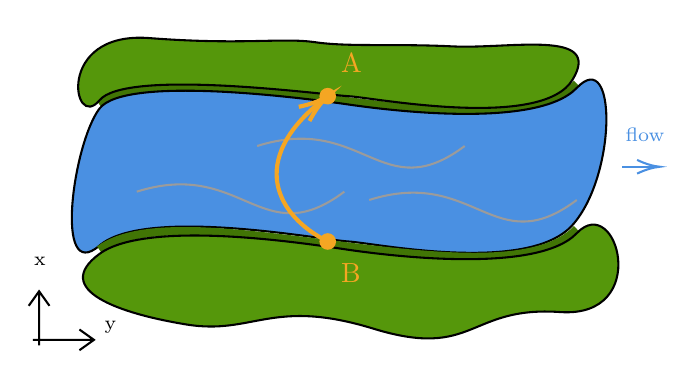
\begin{tikzpicture}[x=0.75pt,y=0.75pt,yscale=-1,xscale=1]
    %uncomment if require: \path (0,300); %set diagram left start at 0, and has height of 300
    
    %Curve Lines [id:da608977851192717] 
    \draw [color={rgb, 255:red, 65; green, 117; blue, 5 }  ,draw opacity=1 ][line width=3]    (300,110) .. controls (340,80) and (493.51,138.06) .. (530,100) ;
    %Shape: Polygon Curved [id:ds9392726871646548] 
    \draw  [fill={rgb, 255:red, 74; green, 144; blue, 226 }  ,fill opacity=1 ] (300,112) .. controls (312.68,95.2) and (403.92,107.66) .. (420,110) .. controls (436.08,112.34) and (510.65,122.34) .. (530,102) .. controls (549.35,81.66) and (549.3,143.91) .. (528,168) .. controls (506.7,192.09) and (432.13,176.66) .. (420,176) .. controls (407.87,175.34) and (322.13,158.94) .. (300,178) .. controls (277.87,197.06) and (287.32,128.8) .. (300,112) -- cycle ;
    %Curve Lines [id:da6433547723995421] 
    \draw [color={rgb, 255:red, 65; green, 117; blue, 5 }  ,draw opacity=1 ][line width=3]    (300,180) .. controls (340,150) and (493.51,208.06) .. (530,170) ;
    %Shape: Polygon Curved [id:ds34371397326569686] 
    \draw  [fill={rgb, 255:red, 85; green, 151; blue, 11 }  ,fill opacity=1 ] (300,182) .. controls (323.56,164.66) and (403.92,177.66) .. (420,180) .. controls (436.08,182.34) and (510.65,192.34) .. (530,172) .. controls (549.35,151.66) and (566.44,213.06) .. (522,210) .. controls (477.56,206.94) and (481.01,233.06) .. (432,218) .. controls (382.99,202.94) and (374.13,221.23) .. (342,216) .. controls (309.87,210.77) and (276.44,199.34) .. (300,182) -- cycle ;
    %Shape: Polygon Curved [id:ds3342416894164969] 
    \draw  [fill={rgb, 255:red, 85; green, 151; blue, 11 }  ,fill opacity=1 ] (324,78) .. controls (369.58,81.49) and (387.92,77.66) .. (404,80) .. controls (420.08,82.34) and (442.15,80.63) .. (470,82) .. controls (497.85,83.37) and (542.72,73.49) .. (528,98) .. controls (513.28,122.51) and (432.13,106.66) .. (420,106) .. controls (407.87,105.34) and (312.7,92.51) .. (300,108) .. controls (287.3,123.49) and (278.42,74.51) .. (324,78) -- cycle ;
    %Curve Lines [id:da7504908272245701] 
    \draw [color={rgb, 255:red, 155; green, 155; blue, 155 }  ,draw opacity=1 ]   (318,152) .. controls (369.01,135.91) and (378,182) .. (418,152) ;
    %Curve Lines [id:da01966435364089625] 
    \draw [color={rgb, 255:red, 155; green, 155; blue, 155 }  ,draw opacity=1 ]   (376,130) .. controls (427.01,113.91) and (436,160) .. (476,130) ;
    %Curve Lines [id:da5498107083025197] 
    \draw [color={rgb, 255:red, 155; green, 155; blue, 155 }  ,draw opacity=1 ]   (430,156) .. controls (481.01,139.91) and (490,186) .. (530,156) ;
    %Shape: Circle [id:dp01198373160385724] 
    \draw  [draw opacity=0][fill={rgb, 255:red, 245; green, 166; blue, 35 }  ,fill opacity=1 ] (406,106) .. controls (406,103.79) and (407.79,102) .. (410,102) .. controls (412.21,102) and (414,103.79) .. (414,106) .. controls (414,108.21) and (412.21,110) .. (410,110) .. controls (407.79,110) and (406,108.21) .. (406,106) -- cycle ;
    %Shape: Circle [id:dp6252725126232461] 
    \draw  [draw opacity=0][fill={rgb, 255:red, 245; green, 166; blue, 35 }  ,fill opacity=1 ] (406,176) .. controls (406,173.79) and (407.79,172) .. (410,172) .. controls (412.21,172) and (414,173.79) .. (414,176) .. controls (414,178.21) and (412.21,180) .. (410,180) .. controls (407.79,180) and (406,178.21) .. (406,176) -- cycle ;
    %Straight Lines [id:da006269855405936053] 
    \draw [color={rgb, 255:red, 74; green, 144; blue, 226 }  ,draw opacity=1 ]   (552,140) -- (568,140) ;
    \draw [shift={(570,140)}, rotate = 180] [color={rgb, 255:red, 74; green, 144; blue, 226 }  ,draw opacity=1 ][line width=0.75]    (10.93,-3.29) .. controls (6.95,-1.4) and (3.31,-0.3) .. (0,0) .. controls (3.31,0.3) and (6.95,1.4) .. (10.93,3.29)   ;
    %Shape: Axis 2D [id:dp579588107341299] 
    \draw  (268,223.4) -- (297.36,223.4)(270.94,200) -- (270.94,226) (290.36,218.4) -- (297.36,223.4) -- (290.36,228.4) (265.94,207) -- (270.94,200) -- (275.94,207)  ;
    %Curve Lines [id:da1687299064997403] 
    \draw [color={rgb, 255:red, 245; green, 166; blue, 35 }  ,draw opacity=1 ][line width=1.5]    (410,176) .. controls (385.7,163.93) and (370.61,137.1) .. (407.67,107.8) ;
    \draw [shift={(410,106)}, rotate = 143.13] [color={rgb, 255:red, 245; green, 166; blue, 35 }  ,draw opacity=1 ][line width=1.5]    (14.21,-4.28) .. controls (9.04,-1.82) and (4.3,-0.39) .. (0,0) .. controls (4.3,0.39) and (9.04,1.82) .. (14.21,4.28)   ;
    
    % Text Node
    \draw (415,84) node [anchor=north west][inner sep=0.75pt]  [color={rgb, 255:red, 245; green, 166; blue, 35 }  ,opacity=1 ] [align=left] {A};
    % Text Node
    \draw (415,185) node [anchor=north west][inner sep=0.75pt]  [color={rgb, 255:red, 245; green, 166; blue, 35 }  ,opacity=1 ] [align=left] {B};
    % Text Node
    \draw (552,120) node [anchor=north west][inner sep=0.75pt]  [color={rgb, 255:red, 74; green, 144; blue, 226 }  ,opacity=1 ] [align=left] {{\scriptsize flow}};
    % Text Node
    \draw (267,182) node [anchor=north west][inner sep=0.75pt]  [color={rgb, 255:red, 0; green, 0; blue, 0 }  ,opacity=1 ] [align=left] {{\scriptsize x}};
    % Text Node
    \draw (301,213) node [anchor=north west][inner sep=0.75pt]  [color={rgb, 255:red, 0; green, 0; blue, 0 }  ,opacity=1 ] [align=left] {{\scriptsize y}};
    
    
    \end{tikzpicture}
    

    \caption{Fluss der überquert werden soll. Blau ist der Fluss eingezeichnet und grün das Ufer. Die Strömung geht von liks nach rechts und ist mit dem Pfeil eingezeichnet. Unten links noch ein referenz kordinaten System.}
    \label{fig:river_points}
\end{figure}
